%%%%%%%%%%%%%%%%%%%%%%%%%%%%%%%%%%%%%%%%%
% Jacobs Landscape Poster
% LaTeX Template
% Version 1.0 (29/03/13)
%
% Created by:
% Computational Physics and Biophysics Group, Jacobs University
% https://teamwork.jacobs-university.de:8443/confluence/display/CoPandBiG/LaTeX+Poster
% 
% Further modified by:
% Nathaniel Johnston (nathaniel@njohnston.ca)
%
% This template has been downloaded from:
% http://www.LaTeXTemplates.com
%
% License:
% CC BY-NC-SA 3.0 (http://creativecommons.org/licenses/by-nc-sa/3.0/)
%
%%%%%%%%%%%%%%%%%%%%%%%%%%%%%%%%%%%%%%%%%

%----------------------------------------------------------------------------------------
%	PACKAGES AND OTHER DOCUMENT CONFIGURATIONS
%----------------------------------------------------------------------------------------

\documentclass[final]{beamer}

\usepackage{tikz}
%\usepackage{tikz}
\usepackage{graphicx}
\usepackage[scale=1.24]{beamerposter} % Use the beamerposter package for laying out the poster

\usetheme{confposter} % Use the confposter theme supplied with this template

\setbeamercolor{block title}{fg=ngreen,bg=white} % Colors of the block titles
\setbeamercolor{block body}{fg=black,bg=white} % Colors of the body of blocks
\setbeamercolor{block alerted title}{fg=white,bg=dblue!70} % Colors of the highlighted block titles
\setbeamercolor{block alerted body}{fg=black,bg=dblue!10} % Colors of the body of highlighted blocks
% Many more colors are available for use in beamerthemeconfposter.sty

%-----------------------------------------------------------
% Define the column widths and overall poster size
% To set effective sepwid, onecolwid and twocolwid values, first choose how many columns you want and how much separation you want between columns
% In this template, the separation width chosen is 0.024 of the paper width and a 4-column layout
% onecolwid should therefore be (1-(# of columns+1)*sepwid)/# of columns e.g. (1-(4+1)*0.024)/4 = 0.22
% Set twocolwid to be (2*onecolwid)+sepwid = 0.464
% Set threecolwid to be (3*onecolwid)+2*sepwid = 0.708

\newlength{\sepwid}
\newlength{\onecolwid}
\newlength{\twocolwid}
\newlength{\threecolwid}
\newlength{\leftcolwid}
\newlength{\midcolwid}
\newlength{\rightcolwid}
\setlength{\paperwidth}{48in} % A0 width: 46.8in
\setlength{\paperheight}{36in} % A0 height: 33.1in
\setlength{\sepwid}{0.02\paperwidth} % Separation width (white space) between columns
\setlength{\leftcolwid}{0.2\paperwidth} 
\setlength{\midcolwid}{0.36\paperwidth} 
\setlength{\rightcolwid}{0.36\paperwidth} 
\setlength{\onecolwid}{0.22\paperwidth} % Width of one column
\setlength{\twocolwid}{0.464\paperwidth} % Width of two columns
\setlength{\threecolwid}{0.708\paperwidth} % Width of three columns
\setlength{\topmargin}{-0.5in} % Reduce the top margin size
%-----------------------------------------------------------

\usepackage{graphicx}  % Required for including images

\usepackage{booktabs} % Top and bottom rules for tables
\usepackage{mathtools}
\usepackage{exscale} % otherwise \sum etc are messed up
\usepackage{tcolorbox}
\usepackage{caption}
\setbeamertemplate{caption}[numbered]
\include{poster_defs}
\definecolor{mydarkgreen}{RGB}{10,100,30}
%\include{figure_and_table}
%----------------------------------------------------------------------------------------
%	TITLE SECTION 
%----------------------------------------------------------------------------------------
\title{\LARGE Generating with Confidence: Uncertainty Quantification for Black-box Large Language Models} % Poster title

\author[zhenlin4@illinois.edu]{Zhen Lin$^1$ \hspace{4cm} Shubhendu Trivedi \hspace{4cm} Jimeng Sun$^{1,2}$}
\institute[UIUC]
{\hspace{4cm} $^1$ University of Illinois at Urbana-Champaign, $^2$ Carle Illinois College of Medicine}

\input{poster_resources/defs_poster}

%----------------------------------------------------------------------------------------


\begin{document}

%-----------LOGO ADDED TO NORTH EAST----------------%
\addtobeamertemplate{headline}{} 
{\begin{tikzpicture}[remember picture, overlay]
     \node [anchor=north east, inner sep=9cm]  at (current page.north east)
     {
\includegraphics[height=3.5cm]{poster_resources/illinois_logo.png}};
  \end{tikzpicture}}
%-------END LOGO ADDED TO NORTH EAST----------------%

%-----------LOGO ADDED TO NORTH WEST----------------%
\addtobeamertemplate{headline}{} 
{\begin{tikzpicture}[remember picture, overlay]
     \node [anchor=north west, inner sep=7.5cm] (node_1) at (current page.north west)
     {
\includegraphics[height=6cm]{poster_resources/github_QR.png}
     
\includegraphics[height=6cm]{poster_resources/sunlab.png}};
  % Add "code" text under the QR.png
  \node [font=\Large,xshift=5cm] at (node_1.west) {github:};
  \end{tikzpicture}}
 %-------END LOGO ADDED TO NORTH WEST----------------%

\addtobeamertemplate{block end}{}{\vspace*{2ex}} % White space under blocks
\addtobeamertemplate{block alerted end}{}{\vspace*{2ex}} % White space under highlighted (alert) blocks

\setlength{\belowcaptionskip}{2ex} % White space under figures
\setlength\belowdisplayshortskip{2ex} % White space under equations

\begin{frame}[containsverbatim,t] % The whole poster is enclosed in one beamer frame

\begin{columns}[t] % The whole poster consists of three major columns, the second of which is split into two columns twice - the [t] option aligns each column's content to the top

\begin{column}{\sepwid}\end{column} % Empty spacer column

\begin{column}{\leftcolwid} % The first column


\begin{alertblock}{Highlights}

\begin{itemize}
\item We propose confidence and uncertainty estimators, via only \textbf{black-box} LM 
 access.

\item 
We construct semantic similarity matrices from sampled responses to derive uncertainty and confidence estimates.

\item %On popular free-form QA tasks, our black-box uncertainty and confidence measures often outperform white-box baselines
Our black-box uncertainty and confidence measures often outperform white-box baselines on free-form QA tasks.

\end{itemize}

\end{alertblock}

%----------------------------------------------------------------------------------------
%	INTRODUCTION
%----------------------------------------------------------------------------------------
% \begin{block}{\color{mydarkgreen}{Motivation}}
% \begin{itemize}

% \item LLMs often generate high-quality responses—but how confident should we be?

% \item Existing UQ approaches often assume white-box access (e.g., logits), which is unrealistic for closed-source APIs.

% \item We aim to develop simple, effective UQ techniques for black-box LLMs, especially for QA tasks.

% \end{itemize}
% \end{block}


\begin{block}{\color{mydarkgreen}{Uncertainty vs Confidence}}

\begin{itemize}
    \item 
    Given input (prompt) $\mathbf{x}$, the LM $\mathcal{M}$ generate a random response  $\mathbf{s}_j$ with tokens $[s_{j,1},\ldots,s_{j,n_i}]$.
    
    \item \textbf{Confidence} is a property of both the predictive distribution and a particular generation, taking the form of $C(\mathbf{x},\mathbf{s}|\mathcal{M})$.
    Think ``probability'', e.g. sequence probability % $\hat{p}(\mathbf{s}|\mathbf{x}) = \prod_{i} \hat{p}(s_i | s_{<i}, \mathbf{x})$
    %  Example: sequence probability
    \begin{align}
        %C(\mathbf{x},\mathbf{s}) = 
        \hat{p}(\mathbf{s}|\mathbf{x}) &= \prod_{i} \hat{p}(s_i | s_{<i}, \mathbf{x}) \label{eq:jointproba}
    \end{align}
    
    \item \textbf{Uncertainty} is a property of the predictive \textit{distribution}, taking the form of $U(x|\mathcal{M})$. 
    Think  ``dispersion'', e.g. predictive entropy
    \begin{align}
        %U(\mathbf{x}) = 
        \hat{H}(\mathbf{S}|\mathbf{x}) = 
    -\sum_{\mathbf{s}} \hat{p}(\mathbf{s}|\mathbf{x}) \log{(\hat{p}(\mathbf{s}|\mathbf{x}))} \label{eq:entropy:nlg}
    \end{align}

    
\end{itemize}
% Uncertainty and confidence are sometimes deemed antonyms, but they 
% However, confidence scores typically bear a slightly different meaning, especially outside the Bayesian literature. 
% Specifically $U$ only depends on $x$ and is a property of the predictive \textit{distribution}, the confidence scores are generally associated with both the input and the prediction and can be expressed as $C(x, y)$.
% As a concrete example, for $P(Y|x) = \mathcal{N}(\mu, \sigma^2)$, the variance $\sigma^2$ is an uncertainty measure.
% For a particular prediction $Y=y$, the negative z-score $-\frac{|y-\mu|}{\sigma}$ could be a confidence measure.
% Notice the use of a lower-case $y$ in the notation, instead of a upper-case $Y$ that represents a random variable.
% In the context of classification, one of the simplest and most used confidence measures is just the predicted probability $\hat{p}(Y=y|x)$.
% The corresponding {\bf confidence score} in NLG is the joint probability:
% \begin{align}
%     C(x,\mathbf{s}) = \hat{p}(\mathbf{s}|x) &= \prod_{i} \hat{p}(s_i | s_{<i}, x). \label{eq:jointproba}
% \end{align}
\end{block}



\begin{block}{\color{mydarkgreen}{Method Overview}}

\begin{enumerate}
    \item For a given input $\mathbf{x}$, generate $m$ response samples $\mathbf{s}_1, \ldots, \mathbf{s}_m$.
    \item Calculate the pairwise similarity scores $a(\mathbf{s}_{j_1}, \mathbf{s}_{j_2})$ for these $m$ responses.
    \item Compute an uncertainty estimate $U(\mathbf{x})$ or a confidence score $C(\mathbf{x},\mathbf{s}_j)$ using the similarity values.
\end{enumerate}
\end{block}

\end{column} % End of the first column

\begin{column}{\sepwid}\end{column} % Empty spacer column

\begin{column}{\midcolwid} % Begin a column which is two columns wide (column 2)

%\begin{columns}[t,totalwidth=\twocolwid] % Split up the two columns wide column

\begin{column}{\midcolwid}\vspace{-.6in} % The first column within column 2 (column 2.1)
\begin{block}{\color{mydarkgreen}{Measuring Response Similarities ($a(\mathbf{s}_{j_1}, \mathbf{s}_{j_2})$)}}


% We use two ways to compute the similarity between two responses ($a(\mathbf{s}_{j_1}, \mathbf{s}_{j_2})$).% to compare the similarity between a pair of responses.

\textbf{Jaccard Similarity}:
The Jaccard similarity between two responses $\mathbf{s}_{j_1}$ and $\mathbf{s}_{j_2}$ (considered as sets of words) where $j_1,j_2\in[m]$ is computed as:
\begin{align}
    \affinityJaccard(\mathbf{s}_{j_1}, \mathbf{s}_{j_2}) &= |\mathbf{s}_{j_1} \cap \mathbf{s}_{j_2}|/|\mathbf{s}_{j_1} \cup \mathbf{s}_{j_2}| \in [0,1].
\end{align}
Easy to compute, but fails to capture crucial expressions such as negation.
% Despite the computation efficiency, Jaccard similarity has certain limitations, including the lack of consideration for word order and the inability to capture crucial expressions such as negation.

\textbf{Natural Language Inference (NLI)}:
A NLI classifier predicts whether two responses belong to three distinct classes: entailment, neutral, and contradiction. 
We use either entailment or contradiction to define similarity (using a \texttt{DeBERTa-large}):
\begin{align}
    &\affinityEntail(\mathbf{s}_{j_1},\mathbf{s}_{j_2}) = \hat{p}_{entail}(\mathbf{s}_{j_1}, \mathbf{s}_{j_2})
    &\affinityContradict(\mathbf{s}_{j_1},\mathbf{s}_{j_2}) = 1- \hat{p}_{contra}(\mathbf{s}_{j_1}, \mathbf{s}_{j_2}).
\end{align}

\end{block}
%----------------------------------------------------------------------------------------

\begin{block}{\color{mydarkgreen}{Estimating $U$ and $C$ from Similarities}}


We treat each generated response as one node and define the symmetric adjacency matrix $W = (w_{j_1,j_2})_{j_1,j_2=1,\ldots,m}$ with
$w_{j_1,j_2} = (a_{j_1,j_2}+a_{j_2,j_1})/2$.
The symmetric normalized graph Laplacian is then given by
\begin{align}
    L &\defeq I - D^{-\frac{1}{2}}WD^{-\frac{1}{2}} & 
    % \text{ where }  
    D_{j_1,j_2} & =\begin{cases}\sum_{j'\in[m]} w_{j_1,j'} & (j_1=j_2)\\ 0 & (j_1\neq j_2)\end{cases} \label{eq:D}
\end{align}



\tcolorbox[colback=white, colframe=black, boxrule=1pt]
The \textbf{Sum of Eigenvalues of the Graph Laplacian} approximates the number of distinct semantic ideas, defined by the eigenvalues of $L$: $\lambda_1<\cdots<\lambda_m$
\begin{align}
    U_{\methodEigvClip} &= \sum_{k=1}^m \max(0,1-\lambda_k) \label{eq:eigv}.
\end{align}
% To see the connection, between $U_{\methodEigvClip}$ and $U_{\baselineNumSets}$, we recall the classical theorem:
% \begin{theorem}~\citep{von2007tutorial}\label{thm:connectedcomponent}
%     The multiplicity of the eigenvalue $0$ of $L$ is equal to the number of connected components in the graph represented by $W$.
% \end{theorem}
% In other words, with a binary $W$ (two responses are either connected or not at all), the multiplicity of the zero eigenvalue coincides with the number of semantic sets ($U_{\baselineNumSets}$).
% With a weighted $W$ whose entries are continuous, there is typically only one connected component. 
% However, in spectral clustering, the distribution of the eigenvalues is typically used to determine the number of clusters~\citep{von2007tutorial}\footnote{
% In particular, a ``gap'' between a small eigenvalue $\lambda_k$ to a large one $\lambda_{k+1}$ indicates that there are $k$ clusters.}. 
% An illustration is provided in~\cref{fig:eigv}, with $U_{\methodEigvClip}$ roughly corresponding to the ``number of semantic meanings''.
% In \cref{eq:eigv} we ignore eigenvalues larger than 1 as only the smallest few eigenvalues carry important information about the clusters~\citep{von2007tutorial}.



% \begin{wrapfigure}{l}{0.2\textwidth}
\begin{figure}
    {\centering
    \hspace{-10mm}
    \begin{minipage}{0.27\textwidth}
        \centering
        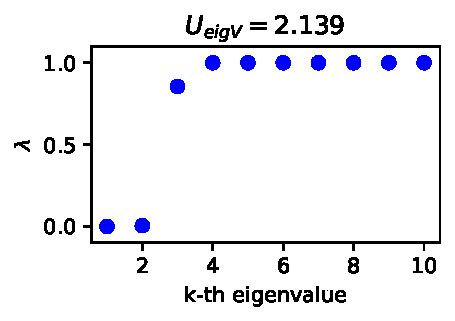
\includegraphics[width=\textwidth]{pics/trivia_low_uq_18_llama.pdf}
    \end{minipage}%\hfill
    \begin{minipage}{0.225\textwidth}
    \scriptsize
    \begin{flushleft}
    \texttt{%
Pink Floyd\\
Pink Floyd in Edinburgh\\
Pink Floyd\\
Shambles\\
Pink Floyd\\
Pink Floyd\\
Pink Floyd\\
Pink Floyd\\
Pink Floyd\\
Pink Floyd%
    }
    \end{flushleft}
\end{minipage}\hspace{-15mm}
    \begin{minipage}{0.27\textwidth}
        \centering
        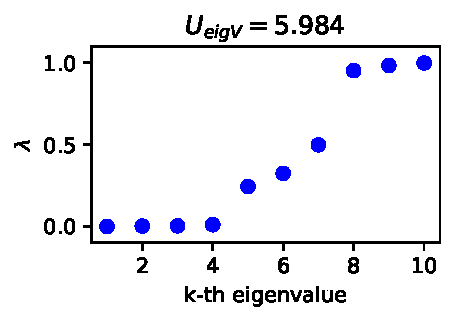
\includegraphics[width=\textwidth]{pics/trivia_high_uq_4_llama.pdf}
    \end{minipage}%\hfill
    \begin{minipage}{0.245\textwidth}
    \scriptsize
    \begin{flushleft}
    \texttt{%
 Leukemia\\
 Low Blood Pressure\\
 Cervical cancer\\
 Cancer in 1953 at 41\\
 Breast cancer\\
 Tuberculosis\\
 Cancer\\
 Leukaemia\\
 Cancer (in 1953 at age 41)\\
 Throat cancer
    }
    \end{flushleft}
\end{minipage}
    }
\begin{minipage}{0.47\textwidth}
   {\scriptsize\textit{Q: Dave Gilmore and Roger Waters were in which rock group?\\ A: Pink Floyd}}
\end{minipage}\hspace{15mm}
\begin{minipage}{0.47\textwidth}
{\scriptsize\textit{Q: What claimed the life of singer Kathleen Ferrier?\\ A: Cancer}}
\end{minipage}
    % \caption{The eigenvalues of the graph Laplacian generated by $\affinityEntail$,  as well as the 10 generated responses and the corresponding $U$.
    % On the left, the question and reference answer are ``Q: Dave Gilmore and Roger Waters were in which rock group? A: Pink Floyd''.
    % We have somewhere between two and three meanings, and $U_{\methodEigvClip}$ is slightly above 2. 
    % The question on the right is ``Q: What claimed the life of singer Kathleen Ferrier? A: Cancer'', and we observe more diverse responses. %, some of which are spelled differently but have similar/the same meanings. 
    % As a result, we see a higher $U_{\methodEigvClip}$ (almost 6).
    % }
    \label{fig:eigv}
\end{figure}
\endtcolorbox


\tcolorbox[colback=white, colframe=black, boxrule=1pt]

\textbf{The Degree Matrix} $D$ can be used directly:
% The previous two methods helped us define the uncertainty $U(x)$ but cannot assign a confidence score to each generated response.
% We utilize the degree matrix $D$ in \cref{eq:D} to define both metrics, as  $D$ already contains relevant information: A node with high degree is well-connected to other nodes, suggesting that it lies in a confident region of the LLM. 
% We thus define uncertainty estimate $U_{\methodDegree}(x)$ and confidence score $C_{\methodDegree}(x, \mathbf{s}_j) $ as
\begin{align}
    &U_{\methodDegree}(x) = trace(mI-D)/m^2
    &C_{\methodDegree}(x, \mathbf{s}_j) = D_{j,j}/m.
\end{align}
\endtcolorbox
% Here, we assume $W_{j_1,j_2}\in[0,1]$.
% $U_{\methodDegree}$ can also be interpreted as the average pairwise distance. 



% \fbox{
% \textbf{Eccentricity} is derived by first computing the spectral embeddings $\mathbf{v}_j$ for each response $\mathbf{s}_j$, and let
% }
% % Recall that one challenge from earlier is that we only have the similarity (or distance) between different responses, but do not know their actual embedding space.
% % The graph Laplacian, however, can provide us with coordinates for the responses.
% % Denote $\mathbf{u}_1, \ldots, \mathbf{u}_k\in\mathbb{R}^m$ as the smallest $k$ eigenvectors of $L$, then an informative embedding of $\mathbf{s}_j$ is simply $\mathbf{v}_j = [u_{1,j},\ldots,u_{k,j}]$~\citep{NIPS2001_801272ee,von2007tutorial}.
% % As a result, we could use the average distance from center as the uncertainty measure, and each response's distance from the center as the (negative) confidence. 
% % Formally, the ``eccentricity'' estimates are:
% \begin{align}
%     & U_{\methodEcc}(x) = \|[\mathbf{v}^{'\top}_1, \ldots, \mathbf{v}^{'\top}_m]\|_2 
%     & C_{\methodEcc}(x, \mathbf{s}_j) = -\|\mathbf{v}'_j\|_2
% \end{align}
% where $\mathbf{v}'_j = \mathbf{v}_j - \frac{1}{m}\sum_{j'=1}^m \mathbf{v}_{j'}$ is normalized by the average embedding.
% \cref{fig:embed} illustrates a sample embedding (from \datasetcoqa).

% \textbf{Remark:}
% The confidence scores $C_{\methodEcc}$ and $C_{\methodDegree}$ in the current form are hardly interpretable.
% For example, $C_{\methodEcc}$ could have a value of 10 or 0.4.
% In practice, they could easily be \textit{calibrated} to match the probability of whether the answer is correct.
% In \cref{appendix:calib} we show that with simple calibration these confidence scores could faithfully reflect the probability of correct answer.



\tcolorbox[colback=white, colframe=black, boxrule=1pt]
{%\centering
    % \hspace{-15mm}
    \begin{minipage}{0.6\textwidth} 
    \leavevmode\noindent
       \textbf{Eccentricity} is derived by first computing the spectral embeddings $\mathbf{v}_j$ for each response $\mathbf{s}_j$, and let
\begin{align}
    & U_{\methodEcc}(x) = \|[\mathbf{v}^{'\top}_1, \ldots, \mathbf{v}^{'\top}_m]\|_2 \\
    & C_{\methodEcc}(x, \mathbf{s}_j) = -\|\mathbf{v}'_j\|_2
\end{align}
where $\mathbf{v}'_j = \mathbf{v}_j - \frac{1}{m}\sum_{j'=1}^m \mathbf{v}_{j'}$ is the centered embedding relative to the mean of all responses.
\end{minipage}
%\hspace{10mm}
    \begin{minipage}{0.37\textwidth}
    \begin{figure}
\centering
\vspace{-1mm}
  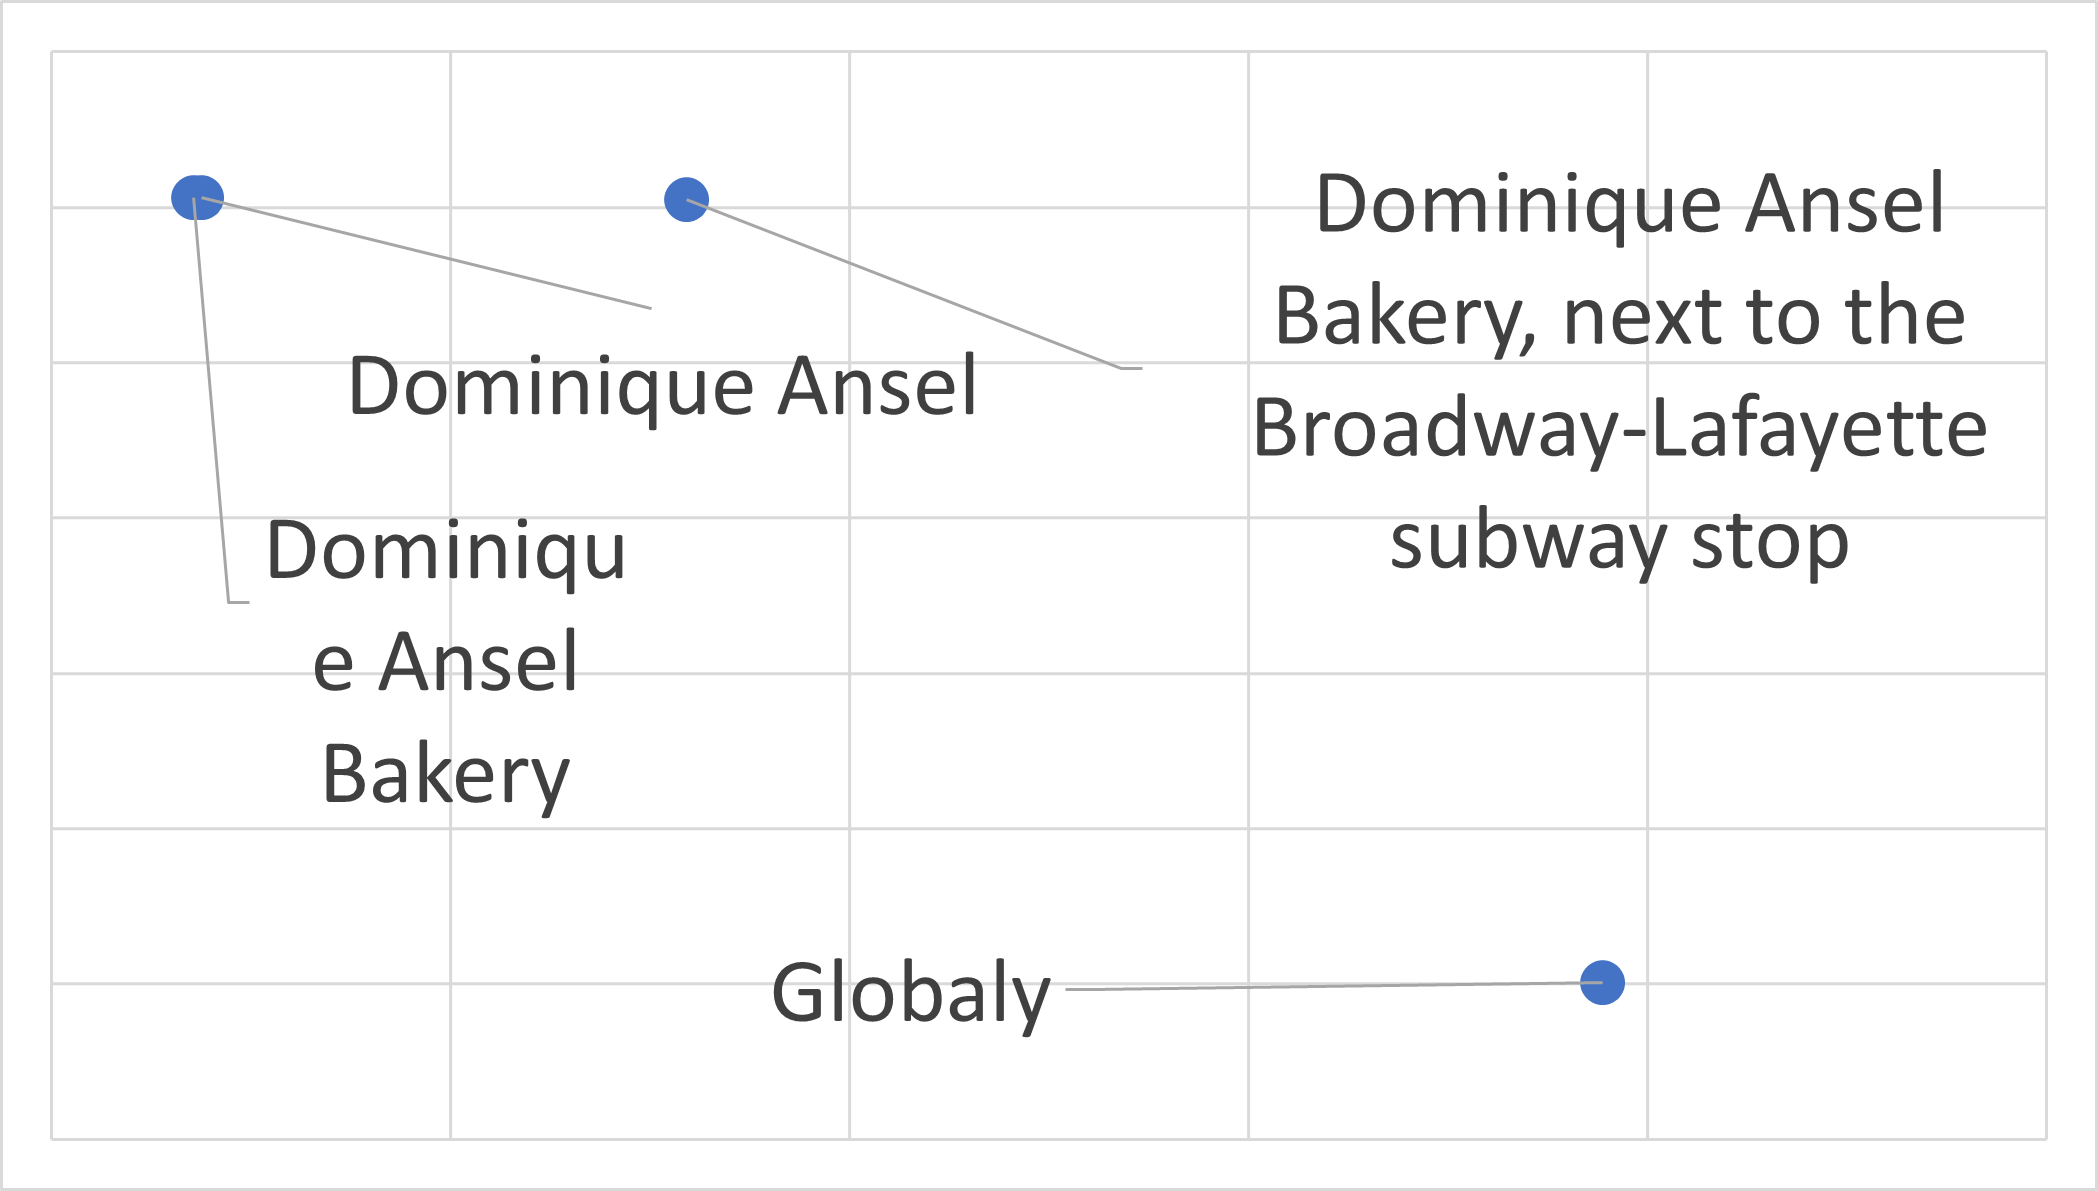
\includegraphics[width=1\textwidth]{pics/embedding.png} 
  \caption{
  % 2D UMAP projection of the e
  Embeddings used in \methodEcc for 20 responses, for ``Q: What is the bakery's name? A:the Dominique Ansel Bakery''.
  % Similar answers tend to live closely together, justifying the use of distance-based uncertainty and confidence measures ($U_\methodEcc$ and $C_\methodEcc$).
  }
  \label{fig:embed}
\end{figure}
\end{minipage}
    }
    \vspace{-10mm}
\endtcolorbox

\end{block}
\end{column} % End of column 2.1

%----------------------------------------------------------------------------------------

\end{column} % End of column 2.2

%\end{columns} % End of the split of column 2

%\end{column} % End of the second column

\begin{column}{\sepwid}\end{column} % Empty spacer column

\begin{column}{\rightcolwid} % The third column


\begin{block}{\color{mydarkgreen}{Experiment Results}}


% \textbf{Datasets}: CoQA (coqa), TriviaQA (trivia), Natural Questions (nq)

% \textbf{Models}:  LLaMA (13B), LLaMA2 (13B), OPT (13B), gpt-3.5-turbo

\textbf{Evaluation Metrics}: 
\begin{itemize}
    \item AUARC: Area under the Accuracy-Rejection Curve. 
    The curve computes the accuracy at each rejection threshold (low-confidence responses or high-uncertainty questions are rejected).
    \item AUROC: $\mathbf{1}\{{\mathbf{s}\text{ correctly answers } \mathbf{x}}\}\sim$ $C(\mathbf{x}, \mathbf{s})$ or $-U(\mathbf{x})$.
\end{itemize}


\begin{figure}[htbp]
  \centering
  \begin{minipage}[b]{0.99\textwidth}
    \centering
    \resizebox{\textwidth}{!}{%
      \begin{tabular}{lc|cccc|cccc|cccc}
\toprule
  &   & trivia(llama) & trivia(llama2) & trivia(opt) & trivia(gpt) & coqa(llama) & coqa(llama2) & coqa(opt) & coqa(gpt) & nq(llama) & nq(llama2) & nq(opt) & nq(gpt)\\
\midrule
\multirow{2}{*}{} & Random & 61.18$\pm$0.07 & 76.24$\pm$0.11 & 25.75$\pm$0.12 & 87.42$\pm$0.08 & 62.46$\pm$0.11 & 78.71$\pm$0.13 & 53.81$\pm$0.18 & 79.76$\pm$0.14 & 23.63$\pm$0.36 & 44.13$\pm$0.68 & 8.60$\pm$0.18 & 62.72$\pm$0.39\\
  & Oracle & 87.03$\pm$0.05 & 96.50$\pm$0.03 & 54.72$\pm$0.19 & 99.09$\pm$0.01 & 86.29$\pm$0.06 & 96.92$\pm$0.03 & 79.41$\pm$0.14 & 97.45$\pm$0.03 & 47.67$\pm$0.55 & 77.62$\pm$0.63 & 23.28$\pm$0.43 & 90.65$\pm$0.21\\
\midrule
\multirow{2}{*}{Baselines} & \baselineNumSets & 78.78$\pm$0.17 & 91.37$\pm$0.12 & 39.46$\pm$0.29 & 93.18$\pm$0.11 & 67.58$\pm$0.17 & 83.66$\pm$0.17 & 60.41$\pm$0.27 & 80.69$\pm$0.22 & 28.18$\pm$0.55 & 57.55$\pm$0.98 & 10.36$\pm$0.27 & 68.92$\pm$0.74\\
  & \baselineLexiSim & 80.32$\pm$0.06 & 91.73$\pm$0.13 & 45.68$\pm$0.24 & 94.69$\pm$0.15 & 78.17$\pm$0.15 & 89.29$\pm$0.16 & 71.46$\pm$0.21 & 86.60$\pm$0.13 & 40.15$\pm$0.70 & 61.88$\pm$1.14 & 15.92$\pm$0.55 & 73.40$\pm$0.74\\
\midrule
\multirow{3}{*}{Ours} & \methodEigvClip(E) & 85.01$\pm$0.08 & \textbf{93.07$\pm$0.17} & 51.54$\pm$0.21 & \underline{\textbf{95.16$\pm$0.21}} & 81.27$\pm$0.12 & \underline{\textbf{90.21$\pm$0.24}} & 73.46$\pm$0.20 & \underline{\textbf{88.80$\pm$0.10}} & \underline{\textbf{40.42$\pm$0.67}} & \underline{\textbf{63.58$\pm$0.96}} & 18.20$\pm$0.44 & \underline{\textbf{75.17$\pm$0.80}}\\
  & \methodEcc(E) & 84.66$\pm$0.06 & \textbf{93.12$\pm$0.12} & 51.42$\pm$0.22 & \underline{\textbf{95.21$\pm$0.22}} & 80.55$\pm$0.14 & \underline{\textbf{90.02$\pm$0.22}} & 72.73$\pm$0.20 & 88.67$\pm$0.13 & 40.38$\pm$0.68 & \underline{\textbf{63.41$\pm$0.92}} & \underline{\textbf{18.82$\pm$0.46}} & \underline{\textbf{75.40$\pm$0.49}}\\
  & \methodDegree(E) & \underline{\textbf{85.27$\pm$0.06}} & \textbf{93.05$\pm$0.14} & \underline{\textbf{52.06$\pm$0.21}} & \underline{\textbf{95.00$\pm$0.23}} & \underline{\textbf{81.50$\pm$0.15}} & \underline{\textbf{90.18$\pm$0.22}} & \underline{\textbf{73.91$\pm$0.19}} & 88.63$\pm$0.23 & \underline{\textbf{41.07$\pm$0.69}} & \underline{\textbf{63.41$\pm$1.03}} & \underline{\textbf{18.43$\pm$0.48}} & 74.35$\pm$0.78\\
\midrule
\multirow{2}{*}{White-box} & \baselineGal & 79.15$\pm$0.08 & \underline{93.99$\pm$0.06} & 51.11$\pm$0.20 & \textendash & 78.83$\pm$0.16 & 89.29$\pm$0.17 & 70.75$\pm$0.21 & \textendash & 36.03$\pm$0.54 & 62.40$\pm$0.98 & \underline{18.40$\pm$0.44} & \textendash\\
  & \baselinePTrue & 64.98$\pm$0.10 & 82.53$\pm$0.09 & 20.25$\pm$0.11 & \textendash & 64.04$\pm$0.18 & 79.92$\pm$0.17 & 50.23$\pm$0.23 & \textendash & 24.72$\pm$0.42 & 44.25$\pm$0.65 & 7.63$\pm$0.22 & \textendash\\
\bottomrule
\bottomrule
\end{tabular}
    }
    \captionof{table}{
    AUARC when using $U(x)$ to predict expected accuracy.
The best black-box methods are in \textbf{bold} and the best overall is \underline{underscored}.
In general, our proposed uncertainty measures perform significantly better than the baselines, sometimes outperforming the white-box methods.
    }
    \label{table:main:exp:arc:u+ea}
  \end{minipage}
\end{figure}


\begin{figure}[htbp]
  \centering
  \begin{minipage}[b]{0.99\textwidth}
    \centering
    \resizebox{\textwidth}{!}{%
      \begin{tabular}{lc|cccc|cccc|cccc}
\toprule
  %& \multicolumn{4}{c}{Baselines}& \multicolumn{9}{|c|}{Ours}& \multicolumn{2}{c}{White-box}\\
    &   & trivia(llama) & trivia(llama2) & trivia(opt) & trivia(gpt) & coqa(llama) & coqa(llama2) & coqa(opt) & coqa(gpt) & nq(llama) & nq(llama2) & nq(opt) & nq(gpt)\\
\midrule
\multirow{2}{*}{} & Random & 61.18$\pm$0.07 & 76.24$\pm$0.11 & 25.75$\pm$0.12 & 87.42$\pm$0.08 & 62.46$\pm$0.11 & 78.71$\pm$0.13 & 53.81$\pm$0.18 & 79.76$\pm$0.14 & 23.63$\pm$0.36 & 44.13$\pm$0.68 & 8.60$\pm$0.18 & 62.72$\pm$0.39\\
  & Oracle & 91.24$\pm$0.03 & 96.92$\pm$0.03 & 60.68$\pm$0.16 & 99.17$\pm$0.01 & 91.85$\pm$0.05 & 97.55$\pm$0.03 & 87.15$\pm$0.11 & 97.80$\pm$0.03 & 57.69$\pm$0.53 & 80.22$\pm$0.56 & 29.65$\pm$0.45 & 91.97$\pm$0.18\\
\midrule
\multirow{2}{*}{Baselines} & \baselineNumSets & 78.78$\pm$0.17 & 91.37$\pm$0.12 & 39.46$\pm$0.29 & 93.18$\pm$0.11 & 67.58$\pm$0.17 & 83.66$\pm$0.17 & 60.41$\pm$0.27 & 80.69$\pm$0.22 & 28.18$\pm$0.55 & 57.55$\pm$0.98 & 10.36$\pm$0.27 & 68.92$\pm$0.74\\
  & \baselineLexiSim & 80.32$\pm$0.06 & 91.73$\pm$0.13 & 45.68$\pm$0.24 & 94.69$\pm$0.15 & 78.17$\pm$0.15 & 89.29$\pm$0.16 & 71.46$\pm$0.21 & 86.60$\pm$0.13 & 40.15$\pm$0.70 & 61.88$\pm$1.14 & 15.92$\pm$0.55 & 73.40$\pm$0.74\\
\midrule
\multirow{3}{*}{Ours} & \methodEigvClip(E) & 85.01$\pm$0.08 & 93.07$\pm$0.17 & 51.54$\pm$0.21 & \underline{\textbf{95.16$\pm$0.21}} & 81.27$\pm$0.12 & \underline{\textbf{90.21$\pm$0.24}} & 73.46$\pm$0.20 & \underline{\textbf{88.80$\pm$0.10}} & 40.42$\pm$0.67 & \underline{\textbf{63.58$\pm$0.96}} & 18.20$\pm$0.44 & \underline{\textbf{75.17$\pm$0.80}}\\
  & \methodEcc(E) & 88.17$\pm$0.11 & \textbf{93.21$\pm$0.07} & 55.82$\pm$0.21 & \underline{\textbf{95.11$\pm$0.18}} & \underline{\textbf{84.62$\pm$0.13}} & \underline{\textbf{90.21$\pm$0.25}} & \underline{\textbf{78.14$\pm$0.20}} & 88.42$\pm$0.19 & 45.78$\pm$0.69 & \underline{\textbf{63.89$\pm$1.08}} & \underline{\textbf{21.00$\pm$0.49}} & \underline{\textbf{75.43$\pm$0.67}}\\
  & \methodDegree(E) & \underline{\textbf{88.86$\pm$0.05}} & \textbf{93.19$\pm$0.11} & \underline{\textbf{56.11$\pm$0.19}} & 94.94$\pm$0.16 & \underline{\textbf{84.60$\pm$0.15}} & 89.75$\pm$0.19 & 77.83$\pm$0.20 & 88.02$\pm$0.31 & \underline{\textbf{46.54$\pm$0.69}} & \underline{\textbf{63.55$\pm$1.01}} & \underline{\textbf{21.30$\pm$0.50}} & 74.67$\pm$0.64\\
\midrule
\multirow{2}{*}{White-box} & \baselineGal & 79.15$\pm$0.08 & \underline{93.99$\pm$0.06} & 51.11$\pm$0.20 & \textendash & 78.83$\pm$0.16 & 89.29$\pm$0.17 & 70.75$\pm$0.21 & \textendash & 36.03$\pm$0.54 & 62.40$\pm$0.98 & 18.40$\pm$0.44 & \textendash\\
  & \baselinePTrue & 67.27$\pm$0.11 & 82.18$\pm$0.08 & 20.89$\pm$0.12 & \textendash & 66.23$\pm$0.19 & 79.55$\pm$0.16 & 49.84$\pm$0.23 & \textendash & 27.62$\pm$0.46 & 44.34$\pm$0.64 & 8.07$\pm$0.21 & \textendash\\
\bottomrule
\end{tabular}
    }
\captionof{table}{
AUARC when using $C(x,\mathbf{s})$ to predict individual accuracy.
AUARC generally improves compared with Table 1.
% The best black-box methods are in \textbf{bold} and the best overall is \underline{underscored}.
% Compared with~\cref{table:main:exp:arc:u+ea}, the AUARC for confidence measures (\methodDegree and \methodEcc) generally improve, as they could discriminate the quality of each response. 
}
\label{table:main:exp:arc:c+ia}
  \end{minipage}
\end{figure}


\begin{figure}[ht]
    \centering
    %\vspace{-3mm}%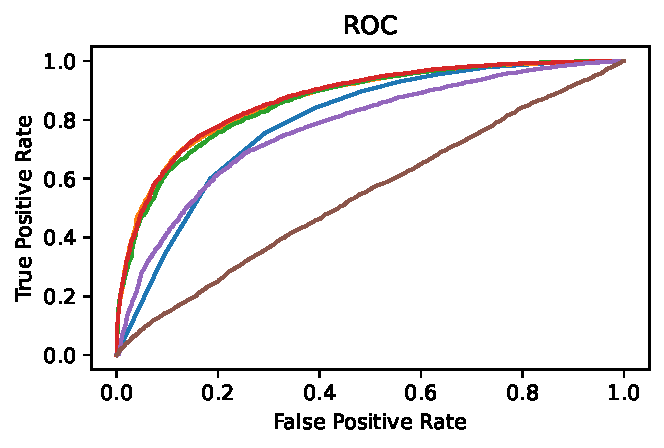
\includegraphics[width=0.45\textwidth]{pics/trivia_llama_auroc.pdf}%
    %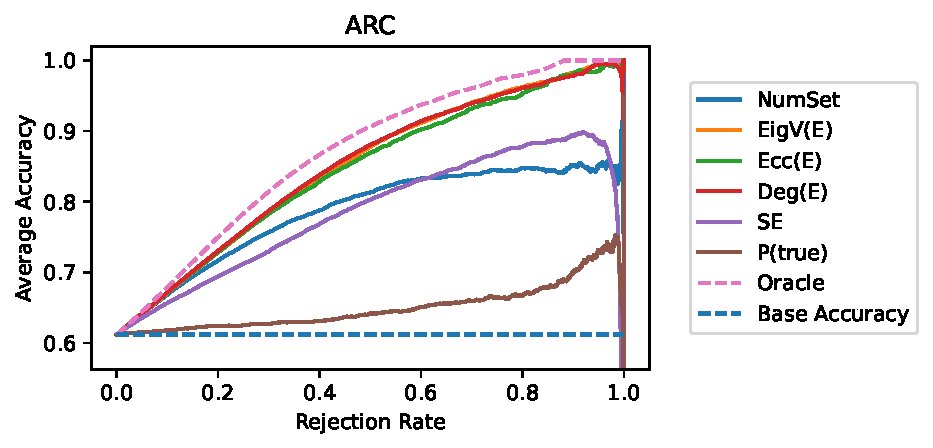
\includegraphics[width=0.45\textwidth]{pics/trivia_llama_auarc.pdf}
    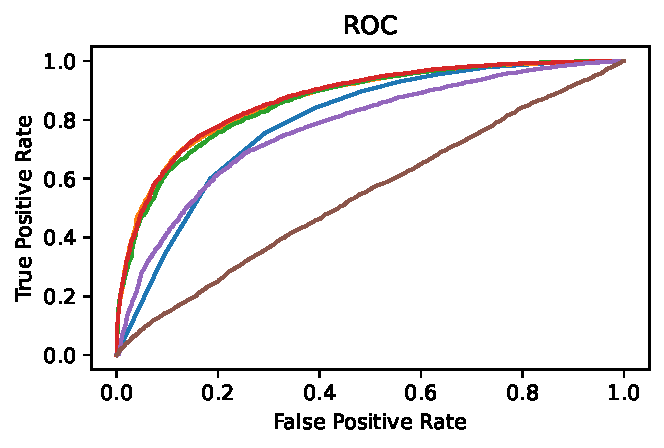
\includegraphics[height=10cm]{pics/trivia_llama_auroc.pdf}%
    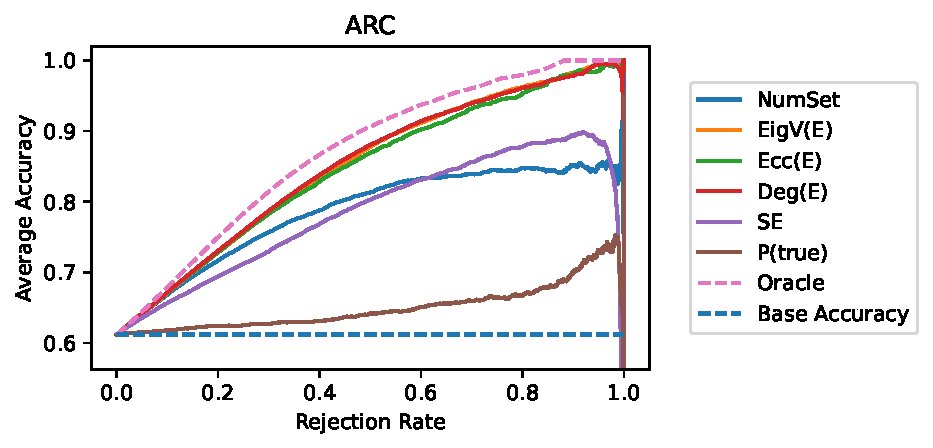
\includegraphics[height=10cm]{pics/trivia_llama_auarc.pdf}
    \caption{The ROC (left) computed using the accuracy of the 1st generated response and the corresponding confidence $C$ (when available, otherwise $U$), for LLaMA on \datasettrivia.
    ARC (right) is computed using $U$ and expected accuracy. 
    % (For ARC, average accuracy is noisy at high rejection rate due to small sample size.) 
    The suffix (E) denotes for $a_{NLI,entail}$. 
    % Different ways to construct $U$ or $C$ from $a_{NLI,entail}$ make a relatively small difference, but are all noticeably better than the baselines (including the white-box baselines).
    % The ARC suggests that if we select only the top 50\% samples using, for example, \methodDegree(E), we could improve the accuracy from 62\% to around 90\%. 
    }
    \label{fig:auroc_auarc}
\end{figure}

\end{block}

%----------------------------------------------------------------------------------------
%	REFERENCES
%----------------------------------------------------------------------------------------

%\begin{block}{References}

%\nocite{*} % Insert publications even if they are not cited in the poster
%\small{\bibliographystyle{unsrt}
%\bibliography{new_poster}\vspace{0.75in}}

%\end{block}

%----------------------------------------------------------------------------------------
%	ACKNOWLEDGEMENTS
%----------------------------------------------------------------------------------------

\setbeamercolor{block title}{fg=red,bg=white} % Change the block title color

\begin{block}{Acknowledgements}

\small{\rmfamily{This work was supported by NSF award SCH-2205289, SCH-2014438, IIS-1838042, NIH award R01 1R01NS107291-01.}} \\

\end{block}

%----------------------------------------------------------------------------------------
%	CONTACT INFORMATION
%----------------------------------------------------------------------------------------

\setbeamercolor{block alerted title}{fg=black,bg=norange} % Change the alert block title colors
\setbeamercolor{block alerted body}{fg=black,bg=white} % Change the alert block body colors

\begin{alertblock}{Additional Information}

\begin{itemize}
\item Code: \href{https://github.com/zlin7/UQ-NLG}{https://github.com/zlin7/UQ-NLG}
\item Email: \href{mailto:zhenlin4@illinois.edu}{zhenlin4@illinois.edu}
\end{itemize}

\end{alertblock}

\end{column} % End of the third column

\end{columns} % End of all the columns in the posterf

\end{frame} % End of the enclosing frame

\end{document}
